\documentclass[authoryear,5p]{elsarticle}

\renewcommand{\today}{}  % Get rid of date on footer
\journal{Ann. Nucl. Energy}

\usepackage[bitstream-charter]{mathdesign} % Use BT Charter font
\usepackage[T1]{fontenc}                   % Use T1 encoding instead of OT1
\usepackage[utf8]{inputenc}                % Use UTF8 input encoding
\usepackage{microtype}                     % Improve typography
\usepackage{amsmath, mathtools}             % AMS Math extensions
\usepackage{booktabs}                      % Improved table spacing
\usepackage{booktabs}
\usepackage{siunitx}
\usepackage{breqn}
\usepackage{nicefrac}

\usepackage[breaklinks=true]{hyperref}

\usepackage{subcaption}
\usepackage{dblfloatfix}
\usepackage{color}

%\usepackage{algorithmic,eqparbox,array}
%\renewcommand\algorithmiccomment[1]{
%  \hspace{\fill}\#\ \eqparbox{COMMENT}{#1}
%}

\usepackage{todonotes}

\usepackage[labelfont=bf]{caption}
\captionsetup[figure]{labelsep=period, name=Figure}
\captionsetup[table]{labelsep=period, name=Table}
\def \figureautorefname {Figure}
\def \algorithmautorefname {Algorithm}

\usepackage[scaled]{beramono}

\usepackage{etoolbox}
\usepackage{listings}
\usepackage{color}

% Algorithm constructs
\usepackage{algorithm} % Provides algorithm environment
\usepackage{algorithmicx}       % Provides algorithmic block
\usepackage{algpseudocode}      % Option of algorithmicx package
\renewcommand{\thealgorithm}{\thechapter-\arabic{algorithm}}
\newcommand\Algphase[1]{%
\vspace*{-.7\baselineskip}\Statex\hspace*{\dimexpr-\algorithmicindent-2pt\relax}\rule{\columnwidth}{0.4pt}%
\Statex\hspace*{-\algorithmicindent}{#1}%
\vspace*{-.7\baselineskip}\Statex\hspace*{\dimexpr-\algorithmicindent-2pt\relax}\rule{\columnwidth}{0.4pt}%
}
\newcommand{\algrule}[1][.4pt]{\par\vskip.5\baselineskip\hrule height #1\par\vskip.5\baselineskip}

\lstset{
  language=Python,
  showstringspaces=false,
  formfeed=\newpage,
  tabsize=4,
  commentstyle=\itshape,
  basicstyle=\ttfamily,
  morekeywords={models, lambda, forms},
  frame=single
}

\newcommand{\code}[2]{
  \subsection*{#1}
  \lstinputlisting{#2}
}

\def\sectionautorefname{Sec.}
\def\subsectionautorefname{Sec.}
\def\subsubsectionautorefname{Sec.}
\def\equationautorefname{Eq.}
\def\figureautorefname{Fig.}
\def\algorithmautorefname{Alg.}

% Patch to make equation autoref counter work
\makeatletter
\patchcmd\eq@setnumber{\stepcounter}{\refstepcounter}{}{%
  \errmessage{Patching \noexpand\eq@setnumber failed}%
}
\makeatother

\hypersetup{colorlinks=true,
  pdftitle={An Analysis of Condensation Errors in Multi-Group Cross-Section Generation for Fine-Mesh Neutron Transport Calculations},
  pdfauthor={William Boyd, Nathan Gibson, Benoit Forget and Kord Smith.}}

\begin{document}

\begin{frontmatter}

\title{An Analysis of Condensation Errors in Multi-Group Cross-Section Generation for Fine-Mesh Neutron Transport Calculations}

\author{William Boyd\corref{cor1}}
\ead{wboyd@mit.edu}

\author{Nathan Gibson\corref{}}
\ead{nathan.gibson@unnpp.gov}

\author{Benoit Forget\corref{}}
\ead{bforget@mit.edu}

\author{Kord Smith\corref{}}
\ead{kord@mit.edu}

\address{Massachusetts Institute of Technology, Department of Nuclear Science and Engineering, 77 Massachusetts Avenue, Building 24, Cambridge, MA 02139, United States\vspace{-8ex}}


%%%%%%%%%%%%%%%%%%%%%%%%%%%%%%%%%%%%%%%%%%%%%%%%%%%%%%%%%%%%%%%%%%%%%%%%%%%%%%%
\begin{abstract}
%%%%%%%%%%%%%%%%%%%%%%%%%%%%%%%%%%%%%%%%%%%%%%%%%%%%%%%%%%%%%%%%%%%%%%%%%%%%%%%

\end{abstract}

\begin{keyword}
Multi-group cross-sections, energy condensation, spatial homogenization, superhomog\'{e}n\'{e}isation factors
\end{keyword}

\end{frontmatter}

%
%%%%%%%%%%%%%%%%%%%%%%%%%%%%%%%%%%%%%%%%%%%%%%%%%%%%%%%%%%%%%%%%%%%%%%%%%%%%%%%%
%\section*{Ben's Outline}
%%%%%%%%%%%%%%%%%%%%%%%%%%%%%%%%%%%%%%%%%%%%%%%%%%%%%%%%%%%%%%%%%%%%%%%%%%%%%%%%

%\begin{itemize}
%\item Problem Statement
%\begin{itemize}
%\item Cross section collapse cannot preserve reaction rates
%\item SPH factors, heterogeneity factors, discontinuity factors
%\end{itemize}
%\item 1D analysis (or 2D Fake)
%\begin{itemize}
%\item Methodology for you 1D slab with single square/SLBW resonance (MOC/CPM solver)
%\item Tables of error by
%\begin{itemize}
%\item resonance peak
%\item resonance width
%\item group width
%\end{itemize}
%\item Angular dependent xs coupled with spatial discretization
%\end{itemize}
%\item 2D analysis (or 2D Real)
%\begin{itemize}
%\item Continuous energy, multi-nuclide, 4 region pin cell
%\item show bias for 2-70 groups (CASMO structures)
%\begin{itemize}
%\item Full OpenMC
%\item Iso-in-lab
%\item Spatial discretization
%\item show effect of discretizing resonance
%\end{itemize}
%\item look at groupwise flux and pcm errors by region, isotope
%\item fixed source OpenMC-OpenMOC shows same phenomenon
%\item SPH factors from OpenMOC by group/region
%\end{itemize}
%\item Possible solutions
%\begin{itemize}
%\item Angular dependent XS
%\item SPH vs just fudging transport xs
%\item Absorption rate in U238 vs SPH factor by resonance group
%\end{itemize}
%\end{itemize}

%%%%%%%%%%%%%%%%%%%%%%%%%%%%%%%%%%%%%%%%%%%%%%%%%%%%%%%%%%%%%%%%%%%%%%%%%%%%%%%
\section{Introduction}
\label{sec:intro}
%%%%%%%%%%%%%%%%%%%%%%%%%%%%%%%%%%%%%%%%%%%%%%%%%%%%%%%%%%%%%%%%%%%%%%%%%%%%%%%

The nuclear reactor physics community has long strived for deterministic neutron transport-based tools for whole-core reactor analysis. A key challenge for whole-core multi-group transport methods is accurate reactor agnostic multi-group cross section (MGXS) generation. The MGXS generation process applies a series of approximations to produce spatially homogenized and energy condensed MGXS in each spatial zone and energy group. Many approximations related to multi-group theory, including the selection of discretized energy group structures and the truncation of the Legendre expansion of the multi-group scattering kernel, are widely studied in the literature. However, the practical impact of the flux separability approximation, which permits the use of the scalar rather than the angular neutron flux to weight the continuous energy cross sections, is less understood. This paper investigates the flux separability approximation and quantifies its significance for heterogeneous PWR problems.

This work employs Monte Carlo (MC) neutron transport simulations to generate MGXS. Monte Carlo methods have increasingly been used to generate few group constants for coarse mesh diffusion, most notably by the Serpent MC code \citep{serpent2013manual}, and to a much lesser extent, for high-fidelity neutron transport methods \citep{redmond1997multigroup, nelson2014improved, cai2014condensation, boyd2016thesis}. The advantage of a MC-based approach is that all of the relevant physics are directly embedded into MGXS by weighting the continuous energy cross sections with a statistical proxy to the ``true'' neutron flux. However, this paper shows that even when the ``true'' scalar flux is used to generate MGXS, the flux separability approximation results in a non-negligible eigenvalue bias between continuous energy and multi-group calculations due to under-prediction of U-238 capture in resonance energy groups.

% In addition, a reference solution may be directly computed from the same MC simulation to compare with the multi-group transport solution.

The content in this paper is organized as follows. The flux separability approximation is introduced in~\autoref{sec:flux-separability}. The methodology used to rigorously quantify the impact of the approximation on PWR problems -- including two benchmark problems and simulation tools -- are described in~\autoref{sec:methodology}. \autoref{sec:test-case1} presents a toy problem which illustrates how scalar flux-weighting of the cross sections cannot preserve the reaction rate for a single resonant energy group, while \autoref{sec:test-case2} investigates the flux separability approximation in the context of a fully-detailed, critical PWR fuel pin cell. SuPerHomog\'{e}n\'{e}isation (SPH) factors is explored in~\autoref{sec:sph} as one possible solution to this approximation, while other approaches, including angular-dependent MGXS, are outlined in~\autoref{sec:conclusions}.
%%%%%%%%%%%%%%%%%%%%%%%%%%%%%%%%%%%%%%%%%%%%%%%%%%%%%%%%%%%%%%%%%%%%%%%%%%%%%%%
\section{Flux Separability Approximation}
\label{sec:flux-separability}
%%%%%%%%%%%%%%%%%%%%%%%%%%%%%%%%%%%%%%%%%%%%%%%%%%%%%%%%%%%%%%%%%%%%%%%%%%%%%%%

The multi-group approach used to solve the transport equation subdivides the neutron's energy into discrete bins known as energy groups. The energy groups are indexed starting at 1 for high energies and ending with $G$ for the lowest energies of interest. The MGXS are the averages of the corresponding continuous energy cross sections weighted by the angular neutron flux $\psi$ in each energy group:

\begin{dmath}
\label{eqn:sigt-mg}
\Sigma_{t,g}(\mathbf{r},\mathbf{\Omega}) \equiv \frac{\int\displaylimits_{E_{g}}^{E_{g-1}} \Sigma_{t}(\mathbf{r},E)\psi(\mathbf{r},\mathbf{\Omega},E)\mathrm{d}E}{\psi_{g}(\mathbf{r},\mathbf{\Omega})}
\end{dmath}

The angular dependence of the total cross section is often treated with the flux separability approximation. Flux separability makes the simplifying assumption that the energy and angular dependence of the flux varies independently such that the angular flux can be written as the product of the scalar neutron flux $\phi(\mathbf{r},E)$ and some function $W(\mathbf{r}, \mathbf{\Omega})$:

\begin{dmath}
\label{eqn:flux-separate}
\psi(\mathbf{r},\mathbf{\Omega},E) = \phi(\mathbf{r},E) W(\mathbf{r},\mathbf{\Omega})
\end{dmath}

\noindent The angular dependence of the $\Sigma_{t,g}$ may then be eliminated by inserting Eqn.~\ref{eqn:flux-separate} into Eqn.~\ref{eqn:sigt-mg}, factoring out $W(\mathbf{r},\mathbf{\Omega})$ and writing $\Sigma_{t}$ in terms of the scalar flux:

\begin{dmath}
\label{eqn:sigt-mg-scalar}
\Sigma_{t,g}(\mathbf{r}) \equiv \frac{\int\displaylimits_{E_{g}}^{E_{g-1}} \Sigma_{t}(\mathbf{r},E)\phi(\mathbf{r},E)W(\mathbf{r},\mathbf{\Omega})\mathrm{d}E}{\phi_{g}(\mathbf{r})W(\mathbf{r},\mathbf{\Omega})} = \frac{\int\displaylimits_{E_{g}}^{E_{g-1}} \Sigma_{t}(\mathbf{r},E)\phi(\mathbf{r},E)\mathrm{d}E}{\phi_{g}(\mathbf{r})}
\end{dmath}

Although flux separability is a simple and commonly used approach to reduce the complexity of the ``true'' multi-group total cross section, it is not always valid and may not preserve neutron balance.

%%%%%%%%%%%%%%%%%%%%%%%%%%%%%%%%%%%%%%%%%%%%%%%%%%%%%%%%%%%%%%%%%%%%%%%%%%%%%%%
\section{Methodology}
\label{sec:methodology}
%%%%%%%%%%%%%%%%%%%%%%%%%%%%%%%%%%%%%%%%%%%%%%%%%%%%%%%%%%%%%%%%%%%%%%%%%%%%%%%

Two case studies were used to disaggregate the approximation errors inherent to deterministic multi-group transport methods from the component error specific to the flux separability approximation. Ultra-fine deterministic and continuous energy Monte Carlo transport methods were used to collapse multi-group cross sections and generate reference solutions for each case study as discussed in~\autoref{subsec:test-case1} and~\autoref{subsec:test-case2}, respectively. Both case studies modeled a multi-region PWR fuel pin geometry with varying levels of complexity. The two analyses isolate the impact of the flux separability approximation on local reaction rates, as well as demonstrate the compounding effect of errors in each energy group on the $k$-eigenvalue. The following sections discuss the benchmark specifications and simulation tools used by each case study.

% hammer home that all of this is due to heterogeneous effects:


%%%%%%%%%%%%%%%%%%%%%%%%%%%%%%%%%%%%%%%%%%%%%%%%%%%%%%%%%%%%%%%%%%%%%%%%%%%%%%%
\subsection{Test Case 1: Resonance with Slowing Down Source}
\label{subsec:test-case1}

%%%%%%%%%%%%%%%%%%%%%%%%%%%%%%%%%%%%%%%%%%%%%%%%%%%%%%%%%%%%%%%%%%%%%%%%%%%%%%%
\subsubsection{Benchmark Problem}
\label{subsubsec:benchmark-case1}

The first test case modeled a simple benchmark problem in which the reference flux could be computed precisely to demonstrate the existence of errors from approximately collapsing Eqn.~\ref{eqn:transport-eqn-ce} into Eqn.~\ref{eqn:transport-eqn-mg-separate} with the flux separability approximation. The first test case problem consisted of a unit cell of an infinite array of unclad fuel pins. The fuel material contained U-238 with an atom density of 0.022 $\nicefrac{\text{a}}{\text{b-cm}}$ and a purely scattering nuclide with a constant cross section of 0.176 cm\textsuperscript{-1}, an analog to oxygen in UO\textsubscript{2}. The moderator was a pure scatterer with a constant cross section of 1.23 cm\textsuperscript{-1}. The pin radius is 0.4 cm and the pitch was 1.26 cm. The source was given by the scatter source from the narrow resonance approximation:

\begin{dmath}
\label{eqn:test-source-ce}
Q(\mathbf{r},\mathbf{\Omega},E) = \frac{1}{4\pi} \frac{\Sigma_{p}(\mathbf{r})}{E}
\end{dmath}

% do you (instead) have a case where you analyze a single resonance with different peak/widths???

%%%%%%%%%%%%%%%%%%%%%%%%%%%%%%%%%%%%%%%%%%%%%%%%%%%%%%%%%%%%%%%%%%%%%%%%%%%%%%%
\subsubsection{Simulation Tools}
\label{subsubsec:sim-tools-case1}

A reference continuous energy flux was computed for the first test case by solving Eqn.~\ref{eqn:transport-eqn-mg-separate} for each energy point {\color{red}[using a toy MOC code? Spatial and angular discretization?]}. The reference reaction rates in each region were obtained by integrating the flux multiplied by a cross section over an energy range of interest and over the volume of the fuel pin. The total cross section was collapsed using the reference flux according to Eqn.~\ref{eqn:sigt-mg-scalar}, and the source was collapsed as follows:

\begin{dmath}
\label{eqn:test1-source-mg}
Q_{g}(\mathbf{r},\mathbf{\Omega}) = \int\displaylimits_{E_{g}}^{E_{g-1}} Q(\mathbf{r},\mathbf{\Omega},E)\mathrm{d}E
\end{dmath}

Eqn.~\ref{eqn:transport-eqn-mg-separate} was solved using {\color{red}[using a toy MOC code? Spatial and angular discretization?]} the collapsed total cross section and source. The collapsed reaction rate was obtained by volume-integrating the multi-group flux multiplied by the multi-group cross section over the fuel pin. Finally, the reaction rates obtained from the multi-group and reference calculations were compared in each energy group to identify any bias due to the flux separability approximation.


%%%%%%%%%%%%%%%%%%%%%%%%%%%%%%%%%%%%%%%%%%%%%%%%%%%%%%%%%%%%%%%%%%%%%%%%%%%%%%%
\subsection{Test Case 2: A Critical PWR Fuel Pin}
\label{subsec:test-case2}

%%%%%%%%%%%%%%%%%%%%%%%%%%%%%%%%%%%%%%%%%%%%%%%%%%%%%%%%%%%%%%%%%%%%%%%%%%%%%%%
\subsubsection{Benchmark Problem}
\label{subsubsec:benchmark-case2}

The second test case modeled a four-region PWR fuel pin, including  2.4\% UO\textsubscript{2} fuel, helium gap, zircaloy clad and borated light water moderator. This benchmark was derived from the BEAVRS PWR model and the material specifications are detailed by~\cite{horelik2013beavrs}. The geometric specifications are reproduced in~\autoref{table:pin-dimensions}. The benchmark geometry is illustrated in~\autoref{fig:pin-materials}. The fuel and moderator were each discretized into sixteen radial zones for spatial homogenization\footnote{Equal volume radial rings were used in the fuel; equally spaced radial rings were used in the moderator.} as shown in~\autoref{fig:pin-rings} for which unique MGXS were generated and employed in multi-group transport calculations.

\begin{table}[h!]
  \centering
  \caption{2D fuel pin dimensions.}
  \label{table:pin-dimensions} 
  \begin{tabular}{l c}
  \toprule
  \multicolumn{1}{c}{\bf Material} &
  {\bf Dimension [cm]} \\
  \midrule
  Fuel Outer Radius & 0.39218 \\
  Gap Outer Radius &  0.40005 \\
  Clad Outer Radius & 0.45720 \\
  Pin Pitch &         1.25984 \\
  \bottomrule
\end{tabular}
\end{table}

\begin{figure}[h!]
\centering
\begin{subfigure}{.25\textwidth}
  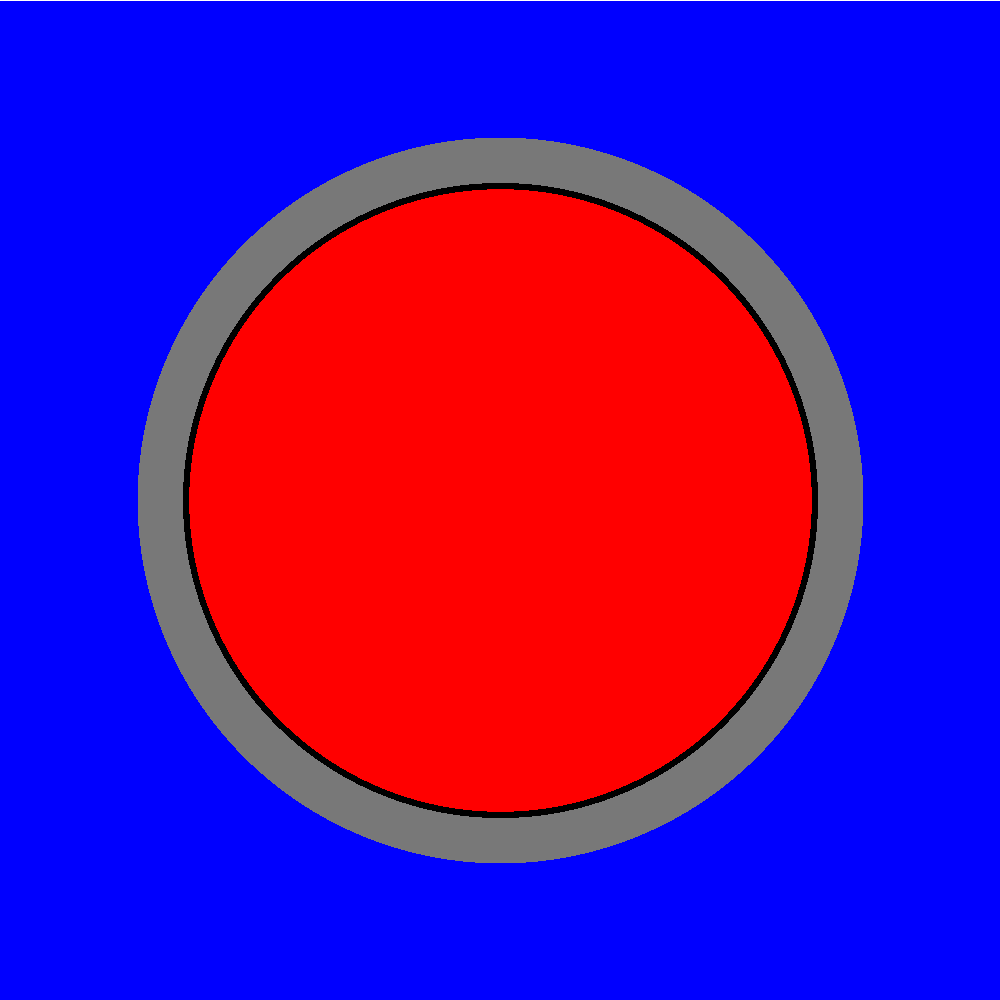
\includegraphics[width=0.9\linewidth]{figures/pin-cell-simple}
  \caption{}
  \label{fig:pin-materials}
\end{subfigure}%
\begin{subfigure}{.25\textwidth}
  \centering
  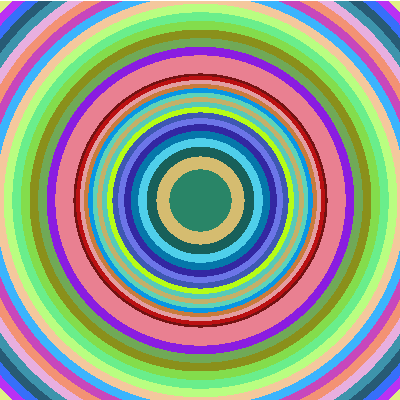
\includegraphics[width=0.9\linewidth]{figures/pin-cell-16x1}
  \caption{}
  \label{fig:pin-rings}
\end{subfigure}
\caption{The PWR fuel pin cell materials (a) and MGXS spatial homogenization zones (b) for the second test case benchmark.}
\label{fig:pin-cell}
\end{figure}

%%%%%%%%%%%%%%%%%%%%%%%%%%%%%%%%%%%%%%%%%%%%%%%%%%%%%%%%%%%%%%%%%%%%%%%%%%%%%%%
\subsection{Simulation Tools}
\label{subsubsec:sim-tools-case2}

The OpenMC continuous energy Monte Carlo code~\citep{romano2013openmc} was employed to generate multi-group cross sections, and reference multi-group reaction rates and fluxes, for the second test case. The \texttt{openmc.mgxs} Python module was used to tally multi-group cross sections in CASMO's seventy energy group structure~\citep{rhodes2006casmo} for each of the radial spatial zones illustrated in Fig.~\ref{fig:pin-rings} from a single eigenvalue calculation. The MGXS were tallied using the scalar flux (Eqn.~\ref{eqn:sigt-mg-scalar}) according to the flux separability approximation. The same Monte Carlo simulation was used to compute a reference eigenvalue, as well as reference multi-group fluxes and reaction rates for each energy group and spatial region. A total of 10 active and 100 inactive batches of 10\textsuperscript{6} particles per batch were simulated. 

The OpenMOC multi-group code~\citep{boyd2014openmoc} was employed to model the second test case benchmark using the MGXS generated by OpenMC. The OpenMOC code is a 2D deterministic method of characteristics code designed for fixed source and eigenvalue neutron transport calculations. The benchmark geometry illustrated in Fig.~\ref{fig:pin-rings} was further discretized for OpenMOC's transport solver with eight azimuthal sectors within each radial ring. A series of multi-group calculations were performed with OpenMOC using the 70-group MGXS tabulated by OpenMC and subsequently collapsed into 1, 2, 8, 16, 25, 40 coarse energy groups. Finally, the OpenMOC eigenvalue and multi-group fluxes were compared with the reference solution computed by OpenMC.

It should be noted that two different OpenMC simulations were performed with different scattering kernels to generate two different MGXS libraries for OpenMOC. The first simulation employed all of the normal scattering physics modeled in OpenMC. The second simulation used OpenMC's ``iso-in-lab'' feature\footnote{The OpenMC ``iso-in-lab'' feature samples the outgoing neutron energy from the scattering laws prescribed by the continuous energy cross section library, but the outgoing neutron direction of motion is sampled from an isotropic in lab distribution.} to enforce isotropic in lab scattering. Although isotropic scattering is not a valid approximation for nuclear reactors, the ``iso-in-lab'' feature enabled comparisons between the reference eigenvalues and reaction rates produced by OpenMC and those computed from isotropic multi-group calculations with OpenMOC. Furthmore, the separate calculations enabled a comparison of the effects due to isotropic in lab scattering and the flux separability approximation.
%%%%%%%%%%%%%%%%%%%%%%%%%%%%%%%%%%%%%%%%%%%%%%%%%%%%%%%%%%%%%%%%%%%%%%%%%%%%%%%
\section{Test Case 1}
\label{sec:test-case1}
%%%%%%%%%%%%%%%%%%%%%%%%%%%%%%%%%%%%%%%%%%%%%%%%%%%%%%%%%%%%%%%%%%%%%%%%%%%%%%%

{\color{red} content to come from Nate's thesis, chapter 9?}

\begin{table}[h!]
  \centering
  \caption{U-238 resonance range reaction rates for collapsed cross sections on simple pin-cell {(\color{red}Table 7.1 from Nate's thesis)}.}
  \label{tab:case1-bias} 
  \begin{tabular}{c c c c c}
  \toprule
  Group & $E_{max}$ [eV] & Reference & Condensed & Error [\%] \\
  \midrule
  15 & 9118.00 & 0.12018 & 0.12030 & 0.102 \\
  16 & 5530.00 & 0.11011 & 0.11027 & 0.142 \\
  17 & 3519.10 & 0.11407 & 0.11444 & 0.330 \\
  18 & 2239.45 & 0.10581 & 0.10630 & 0.457 \\
  19 & 1425.10 & 0.11572 & 0.11625 & 0.461 \\
  20 & 906.899 & 0.21110 & 0.21172 & 0.294 \\
  21 & 367.263 & 0.22169 & 0.22290 & 0.543 \\
  22 & 148.729 & 0.16551 & 0.16649 & 0.598 \\
  23 & 75.5014 & 0.10569 & 0.10621 & 0.487 \\
  24 & 48.0520 & 0.14256 & 0.14394 & 0.964 \\
  25 & 27.7000 & 0.13732 & 0.13867 & 0.984 \\
  26 & 15.9680 & 0.09348 & 0.09348 & 0.001 \\
  27 & 9.87700 & 0.23567 & 0.23813 & 1.041 \\
  \bottomrule
\end{tabular}
\end{table}

\begin{figure}[h!]
  \centering
  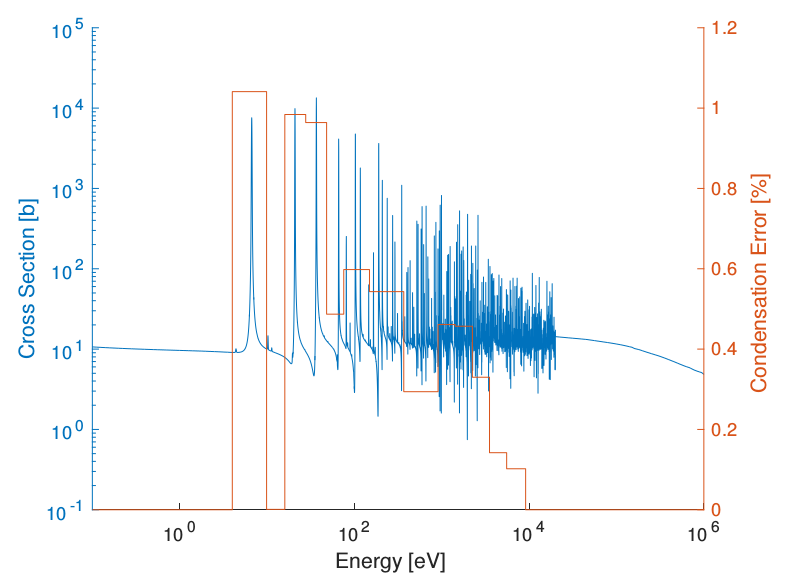
\includegraphics[width=\linewidth]{figures/case1-error}
  \caption{Condensation errors in the resonant groups of the WIMS69 group structure, plotted alongside the U-238 cross section {(\color{red}Figure 7.1 from Nate's thesis)}.}
  \label{fig:case1-errror}
\end{figure}


%%%%%%%%%%%%%%%%%%%%%%%%%%%%%%%%%%%%%%%%%%%%%%%%%%%%%%%%%%%%%%%%%%%%%%%%%%%%%%%
\section{Test Case 2}
\label{sec:test-case2}
%%%%%%%%%%%%%%%%%%%%%%%%%%%%%%%%%%%%%%%%%%%%%%%%%%%%%%%%%%%%%%%%%%%%%%%%%%%%%%%

The second test case was designed to investigate the impact of the groupwise reaction rate errors in the context of an eigenvalue calculation for a PWR benchmark. The influence of the energy-integrated reaction rate errors on the global eigenvalue is evaluated in~\autoref{sec:case2-eigenvalue-bias}, while~\autoref{sec:case2-flux-bias} quantifies the relationship between the bias and reaction rate errors in the energy groups with large resonant capture cross sections.

%%%%%%%%%%%%%%%%%%%%%%%%%%%%%%%%%%%%%%%%%%%%%%%%%%%%%%%%%%%%%%%%%%%%%%%%%%%%%%%
\subsection{Eigenvalue Bias}
\label{sec:case2-eigenvalue-bias}

The OpenMC Monte Carlo code was used to simultaneously tally MGXS in 70 energy groups and compute reference eigenvalues for the second benchmark. The eigenvalues are presented in~\autoref{tab:keff-reference} for simulations with anisotropic scattering, as well as the case when OpenMC's ``iso-in-lab'' feature was employed. The two reference OpenMC simulations were also used to tally separate MGXS libraries to quantify the isotropic in lab scattering approximation used in OpenMOC and to isolate it from the flux separabilty approximation.

\begin{table}[h!]
  \centering
  \caption{Reference OpenMC eigenvalues for a 2D fuel pin.}
  \label{tab:keff-reference} 
  \begin{tabular}{c c}
  \toprule
  {\bf Anisotropic} &
  {\bf Isotropic in Lab} \\
  \midrule
  1.17488 $\pm$ 0.00001 & 1.17422 $\pm$ 0.00001 \\
  \bottomrule
\end{tabular}
\end{table}

The MGXS were employed by a series deterministic multi-group transport simulations to quantify the interaction between the energy and spatial approximations. The effects of energy discretization was analyzed by collapsing the 70-group MGXS library to coarser group structures used by the CASMO code. The MOC Flat Source Region (FSR) spatial discretization meshes were varied with constant-by material MGXS in each FSR to quantify the interaction between the energy and spatial approximations. In particular, 1, 4 or 16 radial rings were used to discretize both the fuel and moderator, while 8 azimuthal sectors were used to discretize the fuel, gap, clad and moderator. The MGXS were computed using tally meshes in OpenMC identical to the FSR meshes used by OpenMOC. All OpenMOC simulations used 128 azimuthal angles and 0.01 cm track spacing for the characteristic track laydown.

%The results underline the complex interactions between discretizations in energy and space which are impacted by the loss of angular information due ot the flux separability approximation. 

In the results that follow, the bias $\Delta\rho$ compares the eigenvalue $k_{eff}^{MOC}$ computed by OpenMOC to that of the reference eigenvalue $k_{eff}^{MC}$ computed by OpenMC in units of pcm:

\begin{equation}
\label{eqn:delta-rho}
\Delta\rho = \left(k_{eff}^{MOC} - k_{eff}^{MC}\right) \times 10^{5}
\end{equation}

\noindent The eigenvalue bias for the ``normal'' anisotropic and ``iso-in-lab'' simulations are presented in~\autoref{tab:keff-bias-aniso} and~\autoref{tab:keff-bias-iso-in-lab}, respectively, for varying energy group structures and FSR spatial discretizations. The results illustrate a strong interaction between the energy and spatial meshes used to solve the multi-group transport equation.

%In particular, the eigenvalue bias grows in magnitude with more energy groups and FSRs but is largely insensitive to the the elimination of the isotropic scattering approximation.

\begin{table}[h!]
  \centering
  \caption{The eigenvalue bias with anisotropic scattering.}
  \label{tab:keff-bias-aniso} 
  \begin{tabular}{c S[table-format=6.1] S[table-format=6.1] S[table-format=6.1]}
  \toprule
  & \multicolumn{3}{c}{{\bf FSR Discretization}} \\
  \cline{2-4}
  \multicolumn{1}{c}{{\bf \# Groups}} &
  {\bf 1$\times$} & {\bf 4$\times$} & {\bf 16$\times$} \\
  \midrule
1 & 67 & 63 & 92 \\
2 & 22 & -56 & -51 \\
4 & -58 & -128 & -135 \\
8 & -75 & -182 & -197 \\
16 & -73 & -190 & -207 \\
25 & -128 & -246 & -268 \\
40 & -131 & -261 & -288 \\
70 & -132 & -267 & -297 \\
  \bottomrule
\end{tabular}
\end{table}

%\begin{table}[h!]
%  \centering
%  \caption{The eigenvalue bias with transport-corrected MGXS.}
%  \label{tab:keff-bias-aniso} 
%  \begin{tabular}{c S[table-format=6.1] S[table-format=6.1] S[table-format=6.1]}
%  \toprule
%  & \multicolumn{3}{c}{{\bf FSR Discretization}} \\
%  \cline{2-4}
%  \multicolumn{1}{c}{{\bf \# Groups}} &
%  {\bf 1$\times$} & {\bf 4$\times$} & {\bf 16$\times$} \\
%  \midrule
%1 & 53 & 75 & 72 \\
%2 & 37 & 1 & 4 \\
%4 & -58 & -92 & -109 \\
%8 & -74 & -145 & -170 \\
%16 & -67 & -154 & -183 \\
%25 & -124 & -221 & -245 \\
%40 & -130 & -238 & -265 \\
%70 & -131 & -281 & -274 \\
%  \bottomrule
%\end{tabular}
%\end{table}

\begin{table}[h!]
  \centering
  \caption{The eigenvalue bias with isotropic-in-lab scattering.}
  \label{tab:keff-bias-iso-in-lab} 
  \begin{tabular}{c S[table-format=6.1] S[table-format=6.1] S[table-format=6.1]}
  \toprule
  & \multicolumn{3}{c}{{\bf FSR Discretization}} \\
  \cline{2-4}
  \multicolumn{1}{c}{{\bf \# Groups}} &
  {\bf 1$\times$} & {\bf 4$\times$} & {\bf 16$\times$} \\
  \midrule
1 & 80 & 55 & 66 \\
2 & 141 & 29 & 34 \\
4 & 27 & -43 & -57 \\
8 & 26 & -85 & -102 \\
16 & 35 & -91 & -111 \\
25 & -31 & -158 & -182 \\
40 & -38 & -174 & -202 \\
70 & -39 & -182 & -211 \\
  \bottomrule
\end{tabular}
\end{table}

In particular, the eigenvalue bias varies by up to 350 pcm between energy group structures and nearly 200 pcm between FSR discretizations. The use of isotropic in lab scattering in OpenMC reduces the magnitude of the bias by up to 100 pcm for seventy energy groups, indicating that the majority of the bias is unrelated to approximation error due to OpenMOC's isotropic in lab scattering kernel. Most importantly, the eigenvalue bias grows in magnitude and turns negative for increasingly fine energy group structures.


This analysis illustrates the counter-intuitive result that the bias between continuous energy Monte Carlo and multi-group deterministic transport may in fact increase in magnitude with more energy groups. Rather, these results illustrate that even when cross sections are collapsed using the ``true'' scalar flux from Monte Carlo, reaction rates are not necessarily preserved. As a result, a non-negligible eigenvalue bias emerges between continuous energy and multi-group transport calculations when increasingly fine energy group and spatial discretization meshes are used.

%  -with enough groups (e.g., ultra-fine), MG and MC eigenvalues should match exactly


%%%%%%%%%%%%%%%%%%%%%%%%%%%%%%%%%%%%%%%%%%%%%%%%%%%%%%%%%%%%%%%%%%%%%%%%%%%%%%%
\subsection{Multi-Group Flux Bias}
\label{sec:case2-flux-bias}

The analysis in~\autoref{sec:test-case1} demonstrated that the flux separability approximation leads to significant reaction rate errors in energy groups with large U-238 capture resonances for a simplified PWR fuel pin. This section investigates how such errors in resonance groups may produce the eigenvalue bias observed between continuous energy and multi-group transport calculations. The analysis in this section corresponds to OpenMOC simulations of the second test case benchmark model with a 16 radial ring FSR discretization mesh in both the fuel and moderator. As in~\autoref{sec:case2-eigenvalue-bias}, the MGXS were tallied by OpenMC directly on the OpenMOC flat source region mesh with isotropic in lab scattering.

The 70-group OpenMOC flux was compared to the reference OpenMC flux, and the percent relative error is illustrated in~\autoref{fig:rel-err-energy}. The error is given for the FSRs nearest and furthest from the moderator, along with the average error across all FSRs in the fuel. The U-238 capture cross section is also shown for comparison purposes. The figure reveals an error of up to 2.5\% in the innermost FSR in groups 24, 25 and 27. These energy groups contain the three largest U-238 capture resonances between 4 and 48.052 eV. The flux errors increase as the energy decreases through the resonance region, and the magnitude of the capture resonances increase. The one notable exception to this is group 26 (4 -- 9.877 eV) which does not include a U-238 capture resonance.

\begin{figure}[h!]
\centering
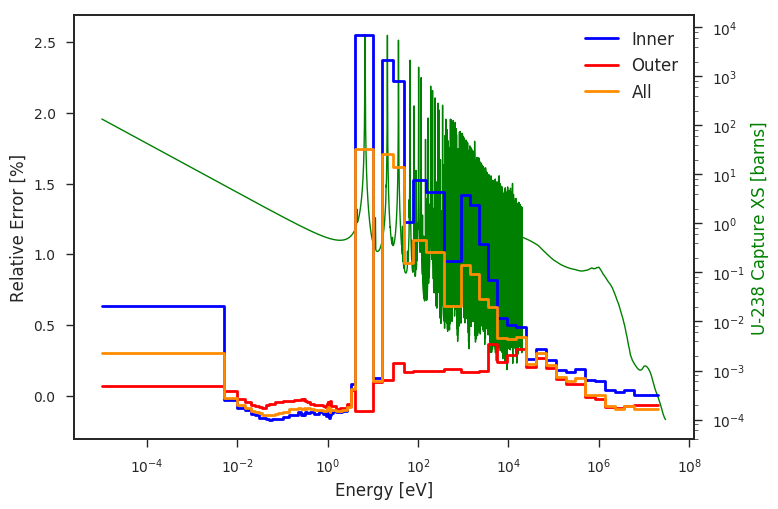
\includegraphics[width=\linewidth]{figures/rel-err-inner-outer}
\caption{The energy-dependent percent relative error of the OpenMOC scalar flux with respect to the reference OpenMC flux for the innermost, outermost and all FSRs.}
\label{fig:rel-err-energy}
\end{figure}

These observations stand in contrast to the flux errors in the outermost FSR for which no remarkable trend can be discerned. The average error across all FSRs is roughly $\nicefrac{2}{3}$ that of the innermost FSR and exhibits the same features in the resonance region. The positive error in the flux in groups with large capture resonances indicates that capture reaction rates are over-predicted in those groups by OpenMOC, contributing to the negative bias in the eigenvalue. Furthermore, these results indicate a strong relationship between the energy and spatial distribution of the flux errors.

The trends in~\autoref{fig:rel-err-energy} indicate a large difference in the error profile for those FSRs nearest and furthest from the moderator. In order to better understand this spatial variation, the flux error was analyzed in the following three energy regimes:

\begin{itemize}
  \item {\bf Range A} -- group 27 encompassing the U-238 capture resonance at 6.67 eV
  \item {\bf Range B} -- groups 11 -- 27 spanning the resonance region from 4 eV -- 408.5 keV
  \item {\bf Range C} -- groups 1 -- 70 spanning the entire energy regime from 0 -- 20 MeV
\end{itemize}

\autoref{fig:rel-err-space} highlights the spatial dependence of the error across the fuel for each energy range. The Range A error monotonically decreases from a maximum of 2.5\% to a minimum near zero in those FSRs furthest and nearest the moderator. Furthermore,  the trend accelerates in the outermost 3 -- 4 FSRs, where the error drops by nearly half of its value at the center of the pin. The error profiles for energy Range B exhibits a similar decreasing trend from the center to the rim of the pin, but the error magnitude never exceeds 0.5\% in magnitude. Finally, the Range C errors do not exhibit a marked trend and are very nearly zero for all flat source regions.

%The systematic error trends in energy and space imply that the negative eigenvalue bias is driven by a poor prediction of the reaction rates in resonance groups, as investigated in the following section.

\begin{figure}[h!]
\centering
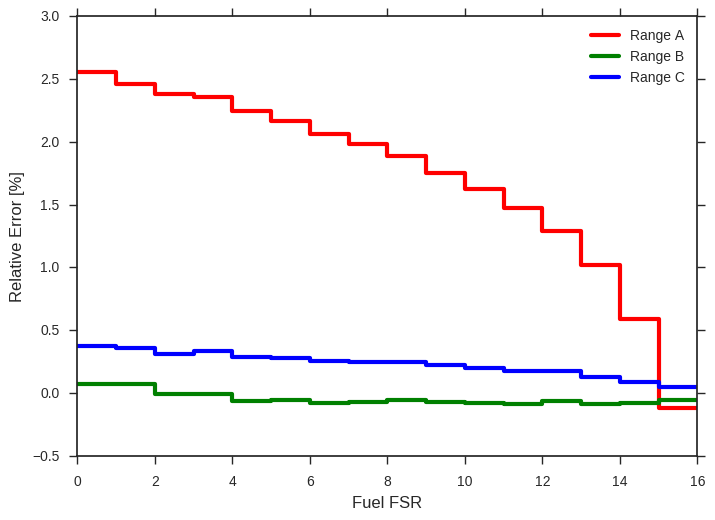
\includegraphics[width=\linewidth]{figures/rel-err-fuel-fsrs}
\caption{The spatially-varying percent relative error of the OpenMOC scalar flux with respect to the reference OpenMC flux in energy Ranges A, B, and C.}
\label{fig:rel-err-space}
\end{figure}

Finally,~\autoref{fig:u238-capture-space} illustrates the spatial dependence of the normalized U-238 capture reaction rates in Range A across the fuel FSRs. The ``rim effect'' of U-238 capture in the outermost ring nearest the moderator is illustrated by the capture rates which are are 5$\times$ greater in the outermost ring than in the innermost rings. The interior zones experience a highly self-shielded flux since neutrons at energies coinciding with the U-238 capture resonance at 6.67 eV are absorbed in the outermost ring before they can further penetrate the fuel. Although the Range A capture rates in the interior regions are relatively small, the largest errors appear in those zones as shown in~\autoref{fig:rel-err-space}. 

\begin{figure}[h!]
\centering
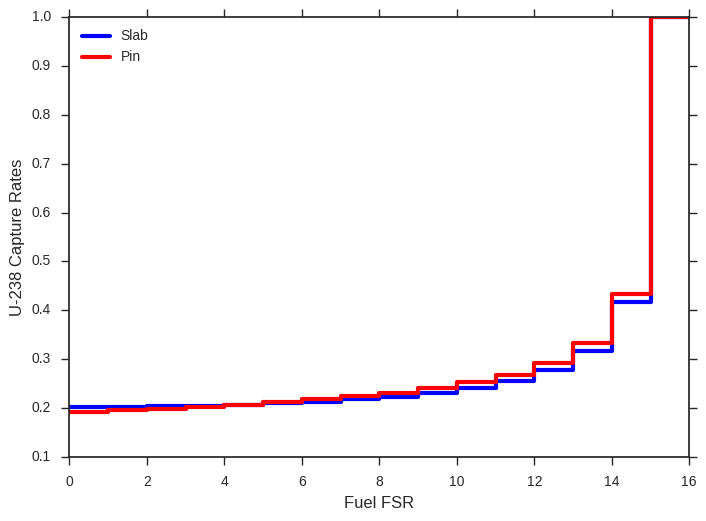
\includegraphics[width=\linewidth]{figures/u238-capt-rates-fuel-fsrs}
\caption{The normalized spatially-varying U-238 capture rates tallied by OpenMC in Range A.}
\label{fig:u238-capture-space}
\end{figure}

These results indicate that spatial self-shielding effects in resonance groups is not adequately captured by the MGXS and/or the multi-group tranport calculation. Although it is challenging to isolate the factors which convolve to bias the eigenvalue, the data presented here demonstrates that an over-prediction of U-238 capture in the resonance groups due to the flux separability approximation is the most important factor.
%%%%%%%%%%%%%%%%%%%%%%%%%%%%%%%%%%%%%%%%%%%%%%%%%%%%%%%%%%%%%%%%%%%%%%%%%%%%%%%
\section{Potential Solutions}
\label{sec:solutions}
%%%%%%%%%%%%%%%%%%%%%%%%%%%%%%%%%%%%%%%%%%%%%%%%%%%%%%%%%%%%%%%%%%%%%%%%%%%%%%%

The preceding sections showed that the flux separability approximation leads to errors in reaction rate errors in energy groups with large U-238 capture resonances, which results in a non-negligible bias in the eigenvalue. This section reviews two approaches to counter the impact of the flux separability approximation. \autoref{subsec:angular-mgxs} investigates the use of angularly-dependent MGXS in the context of the first test case. \autoref{subsec:sph} introduces SuPerHomog\'{e}n\'{e}isation factors to systematically adjust the scalar flux-weighted MGXS to preserve reference reaction rates, in the context of the second test case.

%The preceding results demonstrated that using the ``true'' scalar flux spectrum from an ultra-fine deterministic or Monte Carlo simulation to perform energy condensation and spatial homogenization will not necessarily preserve group reaction rates.


%%%%%%%%%%%%%%%%%%%%%%%%%%%%%%%%%%%%%%%%%%%%%%%%%%%%%%%%%%%%%%%%%%%%%%%%%%%%%%%
\subsection{Angularly-Dependent Total MGXS}
\label{subsec:angular-mgxs}

The flux separability approximation introduced in~\autoref{sec:flux-separability} led to the use of the scalar rather than the angular flux to condense the total cross section in energy. The mathematically proper treatment would instead use the angular flux to condense the total MGXS in angle, energy and space, resulting in angularly-dependent total MGXS. This section shows that using fully angularly-dependent data causes the bias in the group reaction rates to vanish for the first test case benchmark.

As was noted in~\autoref{sec:flux-separability}, the most important aspect of the physics to account for in an LWR fuel pin is whether neutrons are entering the region through the fuel pin or directly from the moderator (see~\autoref{fig:incoming-outgoing}). This self-shielding effect cannot be properly modeled by the simple application of angularly-dependent to a single region fuel pin. In this case, a cross section for a given angle would be applied to both neutrons entering the fuel pin from the moderator and to neutrons exiting the fuel pin on the opposite side. Thus, the fuel pin must also be spatially-discretized in order to resolve the error.

The impact of angularly-dependent MGXS was investigated for first test case benchmark of a simple two-region pin cell. The reference solution was computed on an ultra-fine energy mesh and was used to collapse cross sections. Cross sections for the left hand side of the transport equation were collapsed separately for each angle, weighted by the angular flux for that angle. The geometry was discretized with eight equally-spaced azimuthal sectors. The fuel was split up into three rings of equal volume, while the moderator was subdivided into two equal width rings. {\color{red} How many ultra-fine energy groups? How many discrete angular bins? Include all information necessary to reproduce these results.}

The reaction rate errors in resonance groups with angular flux-weighted MGXS are presented in~\autoref{tab:angular-mgxs-case1}. The results for scalar flux-weighted MGXS given in~\autoref{tab:case1-bias} are reproduced here for clarity. The most significant errors in energy groups 24, 25 and 27 are reduced by up to two orders of magnitude with angularly-dependent MGXS. These results demonstrate that the observed condensation errors can be removed by maintaining fine structure in both angle and space in the condensed cross sections.

\begin{table}[h!]
  \centering
  \caption{U-238 resonance range reaction rate percent relative errors computed with scalar and angular flux-weighted MGXS for the first test case benchmark {(\color{red}Table 7.5 from Nate's thesis)}.}
  \label{tab:angular-mgxs-case1}
  \begin{tabular}{c c c c c}
  \toprule
  & & \multicolumn{2}{c}{\textbf{Error [\%]}} \\
  \cline{3-4}
  \textbf{Group} & \textbf{\boldmath$E_{max}$ [eV]} & \textbf{Scalar} & \textbf{Angular} \\
  \midrule
  15 & 9118.00 & 1.29E-01 & 9.93E-03 \\
  16 & 5530.00 & 1.75E-01 & 1.23E-02 \\
  17 & 3519.10 & 4.04E-01 & 2.68E-02 \\
  18 & 2239.45 & 5.67E-01 & 3.70E-02 \\
  19 & 1425.10 & 5.75E-01 & 3.64E-02 \\
  20 & 906.899 & 3.65E-01 & 2.20E-02 \\
  21 & 367.263 & 6.99E-01 & 4.87E-02 \\
  22 & 148.729 & 7.75E-01 & 5.78E-02 \\
  23 & 75.5014 & 6.47E-01 & 4.90E-02 \\
  24 & 48.0520 & 1.24E+00 & 1.10E-02 \\
  25 & 27.7000 & 1.27E+00 & 1.18E-02 \\
  26 & 15.9680 & 1.29E-03 & 3.45E-02 \\
  27 & 9.87700 & 1.34E+00 & 1.21E-01 \\
  \bottomrule
\end{tabular}
\end{table}

Although this demonstration fully diagnoses the observed errors, this does not suggest that the ultimate solution to condensation errors is to use such fine structure. This would come at a great computational expense, as the spatial discretization increases the cost of the transport solve, and the angularly-dependent cross sections dramatically increase the memory requirements. In addition, flux separability is commonly used since conventional MGXS generation schemes are generally incapable of approximating the angular dependence of the flux in the arbitrary geometries and spatial discretizations modeled by multi-group transport codes.

%As a result, multi-group codes are unable to reproduce the correct angular dependence of the neutron flux with scalar flux-weighted MGXS. Furthermore, flux separability is an approximation which may lead to non-trivial errors in downstream multi-group calculations, such as the eigenvalue bias observed in~\autoref{sec:test-case2}.


%%%%%%%%%%%%%%%%%%%%%%%%%%%%%%%%%%%%%%%%%%%%%%%%%%%%%%%%%%%%%%%%%%%%%%%%%%%%%%%
\subsection{SuPerHomog\'{e}n\'{e}isation Factors}
\label{subsec:sph}

Although angularly-dependent MGXS eliminate the flux separability approximation, they would significantly increase the memory footprint for MGXS libraries and be complicated to accommodate in multi-group transport codes. SuPerHomog\'{e}n\'{e}isation (SPH) factors is an alternative method to reduce heterogeneous resonant reaction rate errors. SPH factors were first proposed by~\cite{hebert1993consistent} to preserve reaction rates during energy condensation and spatial homogenization. SPH factors have traditionally been applied to spatially-homogenized few-group MGXS for coarse mesh diffusion applications. This section introduces SPH factors as an equivalence method between continuous energy Monte Carlo and deterministic multi-group transport methods for the second test case benchmark.

%%%%%%%%%%%%%%%%%%%%%%%%%%%%%%%%%%%%%%%%%%%%%%%%%%%%%%%%%%%%%%%%%%%%%%%%%%%%%%%
\subsubsection{SPH Algorithm}
\label{subsubsec:sph-algorithm}

%SPH is a relatively simple-to-implement method which was evaluated in OpenMOC as discussed in the following sections.

The SPH algorithm enforces reaction rate preservation between a reference fine-mesh transport problem and a corresponding coarse mesh transport or diffusion problem in energy and space. As a result, the SPH factor algorithm requires knowledge of a reference source that is used in a multi-group fixed source solver to derive multiplicative factors that adjust the total MGXS to force neutron balance. In particular, the SPH scheme postulates the existence of a set of factors $\mu_{k,g}$ for each spatial zone $k$ and energy group $g$ which force the streaming and collision terms in the transport equation to balance with a fixed source $Q_{k,g}$:

\begin{dmath}
\label{eqn:sph-transport-eqn}
\mathbf{\Omega} \cdot \nabla \psi_{g}(\mathbf{r},\mathbf{\Omega}) + \mu_{k,g}\Sigma_{t,k,g}\psi_{g}(\mathbf{r},\mathbf{\Omega}) = Q_{k,g}(\mathbf{\Omega})
\end{dmath}

The SPH factors are applied to correct the total MGXS in each region and group. The fixed source $Q_{k,g}$ is computed from the reference fine-mesh solution. In this case, the fixed source is treated as the sum of scattering and fission production sources in each energy group and spatial zone. Given the fixed source and total MGXS from MC,~\autoref{eqn:sph-transport-eqn} may be solved using any multi-group transport method, such as MOC.

%The challenge is to devise estimates to the true SPH factors $\mu_{k,g}$ which adequately preserve reaction rates. 

%For example, continuous energy Monte Carlo can be used to compute reference multi-group fluxes and MGXS, which are then combined to compute an isotropic source as follows:

%\begin{dmath}
%\label{eqn:sph-source}
%Q_{k,g}(\mathbf{\Omega}) = \frac{1}{4\pi} \sum_{g'=1}^{G} \Sigma_{s,k,g' \rightarrow g}\phi_{k,g'} + \frac{\chi_{k,g}}{4\pi k_{eff}}\sum_{g'=1}^{G} \nu\Sigma_{f,k,g'}\phi_{k,g'}
%\end{dmath}

An iterative algorithm is used to estimate SPH factors from a series of multi-group fixed source calculations. First, the estimates $\mu_{k,g}^{(n)}$ at iteration $n$ are introduced as a correction factor for the total cross section in~\autoref{eqn:sph-transport-eqn}:

\begin{dmath}
\label{eqn:sph-transport-eqn-iterate}
\mathbf{\Omega} \cdot \nabla \psi_{g}^{(n)}(\mathbf{r},\mathbf{\Omega}) + \mu_{k,g}^{(n-1)}\Sigma_{t,k,g}\psi_{g}^{(n)}(\mathbf{r},\mathbf{\Omega}) = Q_{k,g}(\mathbf{\Omega})
\end{dmath}

\noindent A multi-group transport code is used to solve~\autoref{eqn:sph-transport-eqn-iterate} with angular and volume integration to compute the scalar flux distribution. The SPH factors $\mu_{k,g}^{(n)}$ are found from the ratio of the reference Monte Carlo scalar flux $\phi_{k,g}^{MC}$ to the flux $\phi_{k,g}^{(n)}$ computed from the fixed source calculation at iteration $n$,

\begin{equation}
\label{eqn:sph-update}
\mu_{k,g}^{(n)} = \frac{\phi_{k,g}^{MC}}{\phi_{k,g}^{(n)}}
\end{equation}

\noindent where the factors are initialized to unity on the first iteration.

The SPH factors are used to find a total MGXS which forces neutron balance in~\autoref{eqn:sph-transport-eqn-iterate}. The initial total MGXS $\Sigma_{t,k,g}^{(0)}$ is computed from the reference MC flux and total reaction rate tallies. The SPH factors are then used to obtain a corrected total MGXS $\Sigma_{t,k,g}^{(n)}$ on each iteration:

\begin{dmath}
\label{eqn:sph-update-sigt}
\Sigma_{t,k,g}^{(n)} = \mu_{k,g}^{(n-1)}\Sigma_{t,k,g}^{(0)}
\end{dmath}

The series of fixed source problems defined by~\autoref{eqn:sph-transport-eqn-iterate} are solved until the SPH factors converge. The scattering matrix and fission production cross section are used to compute the reference fixed source, but are not needed in the iterative scheme defined in Eqn.~\ref{eqn:sph-transport-eqn-iterate}. However, the converged SPH factors must be applied to the scattering matrix and fission production cross sections to produce a fully-corrected MGXS library for downstream eigenvalue calculations.

The SPH iteration algorithm described here is summarized in~\autoref{alg:sph}. As presently posed, there is no unique solution to the set of SPH factors which preserve reaction rates. A unique solution may be found by forcing the factors to be unity in non-fissile zones (\textit{e.g.}, moderator, clad and gap). This approach is motivated by the fact that resonances which lead to self-shielding errors -- such as the U-238 capture resonances -- are generally from isotopes in the fuel. However, the reaction rates in non-fissile zones will not be preserved since the MGXS in these zones remain uncorrected, but these errors are dominated by those in the fuel.

\begin{algorithm}[h]
\caption{SPH Factor Algorithm}
\label{alg:sph}
\begin{algorithmic}[1]
  \State Initialize MGXS from MC tallies
  \State Compute reference source from MC flux and MGXS
  \State Initialize SPH factors to unity
  \While{SPH factors are not converged}
    \State Update total MGXS with SPH factors
    \State Solve fixed source transport problem\footnotemark
    \State Compute new SPH factors
  \EndWhile
  \State Update all MGXS with SPH factors
\end{algorithmic}
\end{algorithm}

\footnotetext{A series of $G$ independent fixed source problems may be solved for each of the $G$ groups. Alternatively, a single fixed source problem may simultaneously solve for all $G$ groups, as is done in OpenMOC.}


%%%%%%%%%%%%%%%%%%%%%%%%%%%%%%%%%%%%%%%%%%%%%%%%%%%%%%%%%%%%%%%%%%%%%%%%%%%%%%%
\subsubsection{Results}
\label{subsubsec:sph-results}

The first test case benchmark was modeled with SPH-corrected MGXS for the FSRs in the fuel and compared to the results presented in~\autoref{sec:test-case2}. The MGXS were computed using isotropic in lab scattering and a spatial tally mesh corresponding to an FSR mesh with 16 radial rings in both fuel and moderator. The OpenMOC fixed source and eigenvalue calculations were performed with 128 azimuthal angles and 0.01 cm track spacing. The OpenMOC fixed source calculations were converged to 10$^{-5}$ on the average FSR scalar flux.

The eigenvalue bias $\Delta\rho$ between OpenMC and OpenMOC for SPH-corrected MGXS is presented in~\autoref{tab:keff-bias-sph}, which can be compared to the bias without SPH in~\autoref{tab:keff-bias-iso-in-lab}. The results illustrate a large reduction in the eigenvalue bias; in particular, the bias of -210 pcm was reduced to just -3 pcm for the finest energy and spatial discretization.

\begin{table}[h!]
  \centering
  \caption{The eigenvalue bias with SPH-corrected MGXS.}
  \label{tab:keff-bias-sph} 
  \begin{tabular}{c S[table-format=6.1] S[table-format=6.1] S[table-format=6.1]}
  \toprule
  & \multicolumn{3}{c}{{\bf FSR Discretization}} \\
  \cline{2-4}
  \multicolumn{1}{c}{{\bf \# Groups}} &
  {\bf 1$\times$} & {\bf 4$\times$} & {\bf 16$\times$} \\
  \midrule
1 & 19 & -18 & -14 \\
2 & 25 & -14 & -6 \\
4 & 7 & 2 & 1 \\
8 & 4 & -0 & 2 \\
16 & 5 & 0 & 4 \\
25 & 5 & 2 & -1 \\
40 & 4 & 3 & -2 \\
70 & 4 & 2 & -3 \\
  \bottomrule
\end{tabular}
\end{table}

Although these results illustrate much better agreement between OpenMC and OpenMOC, a non-negligible bias remains in most cases. It is postulated that the remaining bias may be due to the fact that the reaction rate balance enforced with SPH factors assumes that the eigenvalue calculation with a multi-group method will produce the same neutron source distribution as continuous energy Monte Carlo. However, the eigenvalue source is not necessarily conserved since approximation errors from spatial and angular discretization will impact the multi-group method's solution.

%In summary, the eigenvalues between continuous energy and multi-group transport calculations will identically match if the multi-group transport method computes the same eigenvalue source with SPH-corrected MGXS as that found by the continuous energy method.

The error of OpenMOC's 70-group flux with respect to the reference OpenMC flux is displayed in~\autoref{fig:rel-err-energy-sph}. The errors are shown for the innermost and outermost FSRs in the fuel, along with the average error across all FSRs in the fuel. The flux error is greatly reduced with SPH-corrected MGXS, and is nearly flat in energy. The improvement in OpenMOC's flux -- especially in those energy groups with large U-238 capture resonances -- is responsible for the reduction in the eigenvalue bias with SPH-corrected MGXS presented in~\autoref{tab:keff-bias-sph}.

\begin{figure}[h!]
\centering
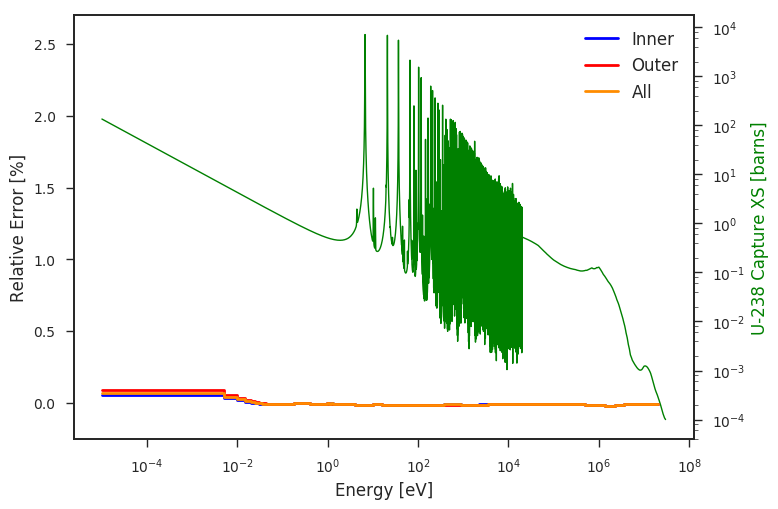
\includegraphics[width=\linewidth]{figures/rel-err-inner-outer-sph}
\caption{The energy-dependent relative error of the OpenMOC scalar flux computed with SPH-corrected MGXS with respect to the reference OpenMC flux for the innermost, outermost and all FSRs.}
\label{fig:rel-err-energy-sph}
\end{figure}

Although SPH factors can greatly improve the agreement between OpenMC and OpenMOC, the SPH approach suffers from a number of shortcomings. First, the SPH approach requires knowledge of the true eigenvalue source distribution. If a reference source must first be computed with a continuous energy method in order to compute SPH-corrected MGXS, then there is no reason to perform a subsequent multi-group calculation since the solution is already known from the reference calculation. Second, the SPH scheme is wholly dependent on the spatial discretization used by downstream deterministic multi-group methods. In particular, the reference source must be calculated from the reference continuous energy method in each of the spatial mesh cells used by the SPH iteration scheme. Lastly, the SPH scheme attempts to preserve reaction rates irregardless of the types of approximation errors which may lead to bias between continuous energy and multi-group transport codes. The SPH scheme simultaneously ``corrects'' the MGXS to account for errors deriving from the spatial, angular and energy discretization and the treatment of the scattering kernel, in addition to those errors resulting from the flux separability approximation.

As a result of the shortcomings to the SPH approach, it is unclear whether the SPH factors may be broadly applied to correct for the flux separability approximation in MGXS generated from MC. Future work should investigate whether a universal set of SPH factors may be tabulated for known geometries (\textit{e.g.}, PWR fuel pins). For example, if the SPH factors in the resonance groups are relatively invariant to the fuel enrichment, moderator density, burnup  and neighboring pin types, then a single set of SPH factors may be computed for an infinite pin cell and applied to each fuel pin in heterogeneous PWR lattice and full-core calculations.

%n particular, the SPH scheme requires knowledge of the reference source distribution, is dependent on the spatial discretization mesh, and is indiscriminate between various sources of approximation error.

%%%%%%%%%%%%%%%%%%%%%%%%%%%%%%%%%%%%%%%%%%%%%%%%%%%%%%%%%%%%%%%%%%%%%%%%%%%%%%%
\section{Conclusions}
\label{sec:conclusions}
%%%%%%%%%%%%%%%%%%%%%%%%%%%%%%%%%%%%%%%%%%%%%%%%%%%%%%%%%%%%%%%%%%%%%%%%%%%%%%%

first paragraph: summary of problem
-recall flux separability approx: use of scalar flux rather than angular flux to weight MGXS
-recall first test case: two-region pin cell with slowing down source
  -used ultra-fine deterministic transport reference solution to collapse MGXS
  -reaction rate errors of over 1\% in groups with largest U-238 capture resonances
-recall second test case: critical four-region PWR pin cell
  -used continous energy MC as reference solution to collapse MGXS with scalar flux-weighted MGXS
  -reaction rate errors led to an eigenvalue bias of approximately 200 pcm due to under-prediction of U-238 capture in resonance groups
-energy and spatial dependence of the bias:
  -the bias emerges / grows with more energy groups
  -reaction rate errors are concentrated in the interior of the fuel pin

second paragraph: solutions
-fully angularly-dependent MGXS
  -demonstrated that it resolves the errors for the two-region pin cell benchmark
-SPH factors
  -equivalence method between continuous energy MC and deterministic transport
  -resolved reaction rate errors and eigenvalue bias for the four-region pin cell benchmark
-angularly-dependent MGXS require memory and are not supported by today's transport codes
-SPH factors suffer from shortcomings

In particular, the SPH scheme requires knowledge of the reference source distribution, is dependent on the spatial discretization mesh, and is indiscriminate between various sources of approximation error.

{\color{red} Future work: jump conditions? coarse angularly-dependent MGXS? universal SPH factors?}

%Although it may be possible to universally apply pre-tabulated SPH factors to fixed geometric configurations, it will likely be necessary to develop alternative methods to account for the angular dependence of the total MGXS. For example, the angular dependence of the total MGXS may be adequately embedded into the scattering kernel using the Consistent-P approximation~\cite{bell1967transport}. Alternatively, a coarse set of angular-dependent MGXS may mitigate most of the bias observed between OpenMC and OpenMOC. For example, a simple approximation might model two different total MGXS for neutrons entering or leaving a fuel pin. Although a coarse angular scheme would not capture the high degree of angular variation illustrated in~\autoref{fig:batman-plots}, it might capture enough to adequately resolve the bias. One challenge to this approach would be to define a general way to accommodate different PWR discretizations within each fuel pin cell.
%%%%%%%%%%%%%%%%%%%%%%%%%%%%%%%%%%%%%%%%%%%%%%%%%%%%%%%%%%%%%%%%%%%%%%%%%%%%%%%
\section*{Acknowledgments}
%%%%%%%%%%%%%%%%%%%%%%%%%%%%%%%%%%%%%%%%%%%%%%%%%%%%%%%%%%%%%%%%%%%%%%%%%%%%%%%


This work was supported by the Idaho National Laboratory and the National Science Foundation Graduate Research Fellowship Grant No. 1122374. This research made use of the resources of the High Performance Computing Center at Idaho National Laboratory, which is supported by the Office of Nuclear Energy of the U.S. Department of Energy and the Nuclear Science User Facilities under Contract No. DE-AC07-05ID14517. The authors' note Adam Nelson's correspondence related to his independent work related to angularly-dependent multi-group cross sections generated with OpenMC.


\section*{References}
\bibliography{references}
\bibliographystyle{annals}

\end{document}
